\chapter{Experiments \& Results} 
\label{chapter-experiments} 

Both are experiments on dataset described in previous chapter. Experiment II will be about energy estimation. Experiment III evaluates and analyzes the robustness of the model with and without EMMA.


%----------------------------------------------------------------------------------------
%	SECTION 
%----------------------------------------------------------------------------------------

\section{Pulsar detection}
The models will be trained to detect pulsar stars. In (very) short, pulsar stars are neutron stars emitting radio waves on a periodic time-frame. A summary of the seminal work of \citep{lyon} can be found in Appendix \ref{chapter-dataset}. The thesis can be accessed \href{http://www.scienceguyrob.com/wp-content/uploads/2016/12/WhyArePulsarsHardToFind_Lyon_2016.pdf}{here}\footnote{\url{http://www.scienceguyrob.com/wp-content/uploads/2016/12/WhyArePulsarsHardToFind_Lyon_2016.pdf}} and the dataset \href{https://archive.ics.uci.edu/ml/datasets/HTRU2}{here}\footnote{\url{https://archive.ics.uci.edu/ml/datasets/HTRU2}}.

Short description of two modes (ip and dm) and internal features (mean...).  Explain why detection is difficult. Classification signal/background. Skewed dataset, give numbers.

%----------------------------------------------------------------------------------------
%	SECTION 
%----------------------------------------------------------------------------------------

\section{Corruption}
\begin{itemize}
\item standardize, why? split sets and apply one from train \href{https://stats.stackexchange.com/questions/327294/data-standardization-for-training-and-testing-sets-for-different-scenarios}{error standardize}
\item SNR (see good explanation in pulsar thesis). If greater than 1, signal non-distinguishable. White noise. Explain it is not the same than AE corruption. $ 10\log(\frac{1}{\sigma^2})$
\item on signal and background because we corrupt the whole mode and not the class
\end{itemize}


%----------------------------------------------------------------------------------------
%	SECTION 
%----------------------------------------------------------------------------------------

\section{Experiment II}

\begin{itemize}
\item train-test split
\item AE trained on train-set and then test on test-set
\item matrix with number of signals, ... (eda)
\end{itemize}

Setup: max epochs = 30, batch size = 64, noise DAE = 0.01, d input = 4, n hidden = 12, adam 0.001, sigmoid

\begin{figure}[!h]
\centering
\begin{subfigure}{.5\textwidth}
  \centering
  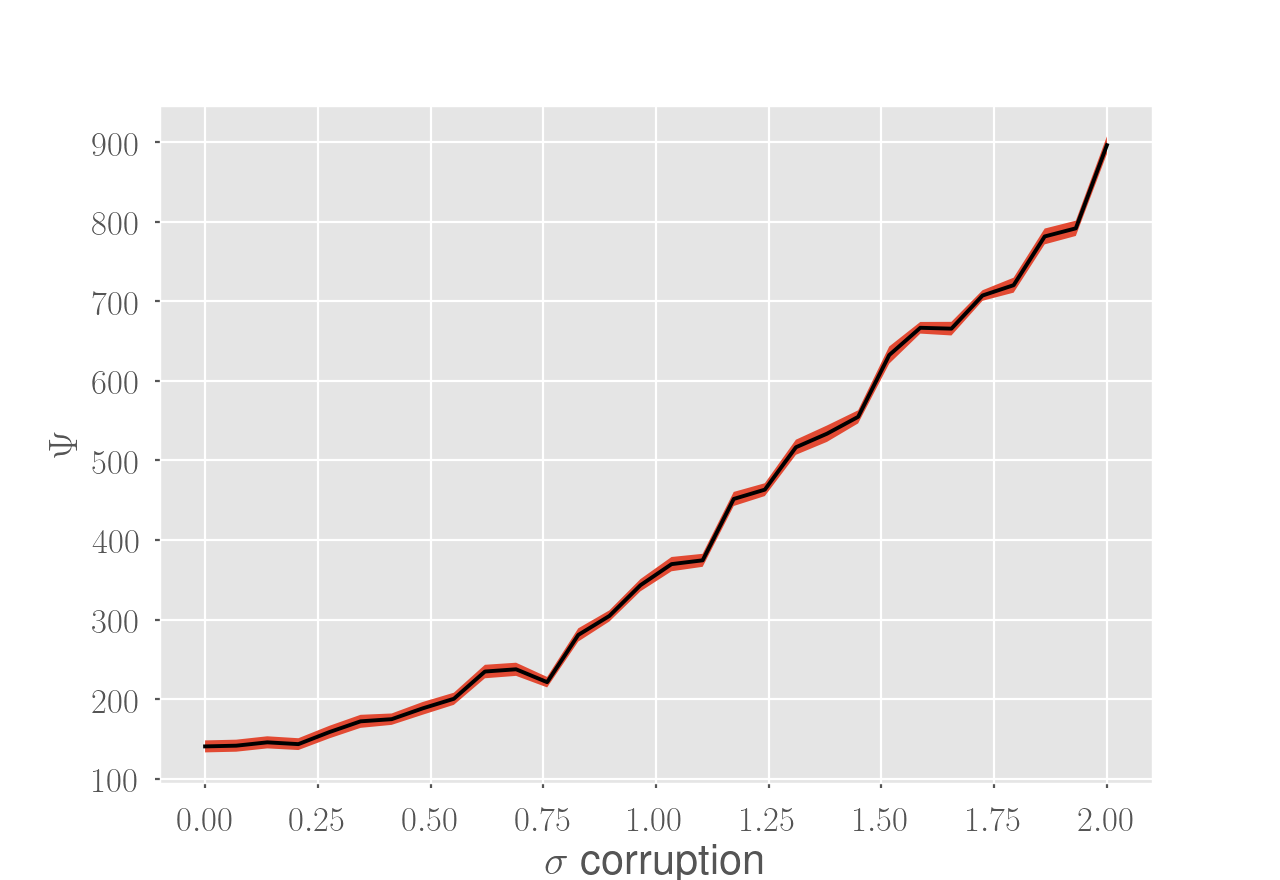
\includegraphics[width=\linewidth]{figures/noisy-signal-ip}
\end{subfigure}%
\begin{subfigure}{.5\textwidth}
  \centering
  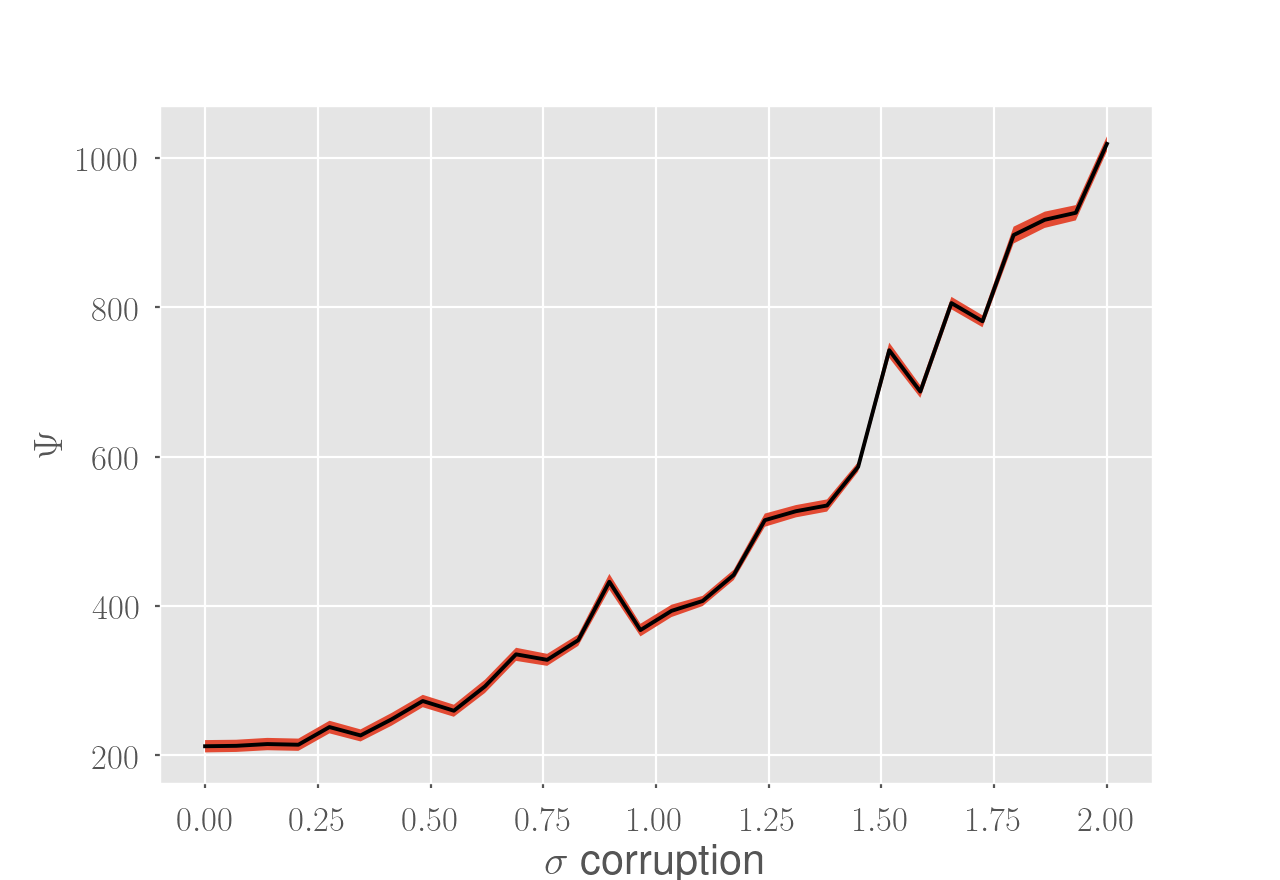
\includegraphics[width=\linewidth]{figures/noisy-signal-dm-snr}
\end{subfigure}
\end{figure}


%----------------------------------------------------------------------------------------
%	SECTION 
%----------------------------------------------------------------------------------------

\section{Experiment III}

\begin{itemize}
\item BCE \& F1 (not AUC -- explain why). \href{https://stats.stackexchange.com/questions/210700/how-to-choose-between-roc-auc-and-f1-score}{F1vsAUC1}. \href{https://www.quora.com/What-does-it-mean-to-have-high-AUC-but-low-F1-score}{F1vsAUC2}. \href{https://stackoverflow.com/questions/44172162/f1-score-vs-roc-auc}{F1vsAUC3}. \href{https://www.mikulskibartosz.name/f1-score-explained/}{F1}
\item train-valid-test
\item threshold optimal choice via ROC. all on valid set
\item 3 models: base (train normal, valid normal), without (train noisy, valid noisy), with (train noisy, valid noisy)
\item 50-25-25 noisy mode. give detailed numbers. eda.
\item trained with early stopping + retrain for .. epochs with valid+train. saved model.
\item one subsection per plot: explain details experiment and how results are obtained. then analyze and conclusions.
\end{itemize}

%\begin{landscape}
%\begin{table}
%\centering
%
%\begin{tabular}{@{}lccccccccc@{}}
%\toprule
%Model &  \multicolumn{3}{c}{$F_1$-Scores} & \multicolumn{3}{c}{Precision} & \multicolumn{3}{c}{Recall}  \\
%\cmidrule(lr){2-4}  \cmidrule(lr){5-7}   \cmidrule(lr){8-10} 
%& uncorrupted & noisy-ip & noisy-dm & uncorrupted & noisy-ip & noisy-dm & uncorrupted & noisy-ip & noisy-dm \\
%\midrule
%Without &  \\ %\cline{1-4}
%\hspace*{\fill}Glasses        & 76.78\% & 70.91\% & 74.17\%& 75.95\% & 76.12\% & 76.04\%& 75.95\% & 76.12\% & 76.04\%  \\ %\cline{1-4}
%With& \\ %\cline{1-4}
%Night-BareFace & 80.66\% & 72.11\% & 77.16\%& 75.95\% & 76.12\% & 76.04\%& 75.95\% & 76.12\% & 76.04\%  \\ %\cline{1-4}
%Night-Glasses  & 74.20\% & 81.66\% & 78.56\%& 75.95\% & 76.12\% & 76.04\% & 75.95\% & 76.12\% & 76.04\% \\ \addlinespace %\cline{1-4}
%Overall        & 75.81\% & 75.65\% & 75.73\%& 75.95\% & 76.12\% & 76.04\%& 75.95\% & 76.12\% & 76.04\% \\ 
%\bottomrule
%\end{tabular}
%\caption{Experimental results}
%\label{my-label}
%\end{table}
%\end{landscape}




  
\subsection*{Attention-shift}
\begin{figure}[!h]
\centering
\begin{subfigure}{.5\textwidth}
  \centering
  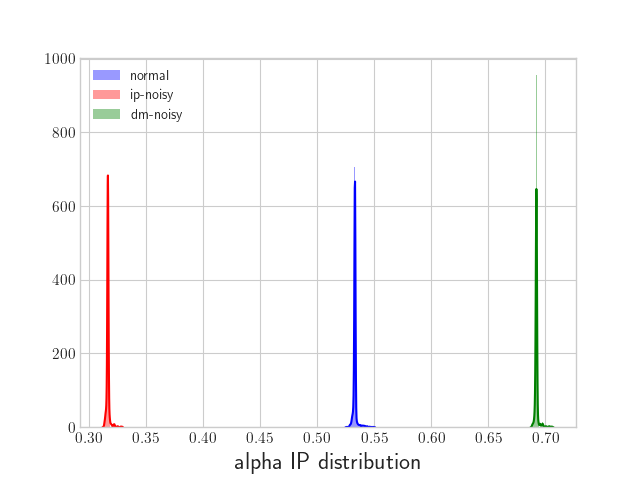
\includegraphics[width=\linewidth]{figures/alpha-distrib-high-cap}
\end{subfigure}%
\begin{subfigure}{.5\textwidth}
  \centering
  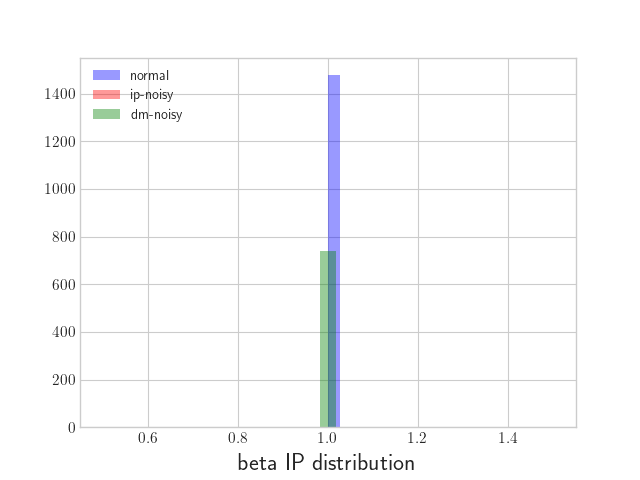
\includegraphics[width=\linewidth]{figures/beta-distrib-high-cap}
\end{subfigure}
\end{figure}

\begin{figure}[!h]
\centering
\begin{subfigure}{.5\textwidth}
  \centering
  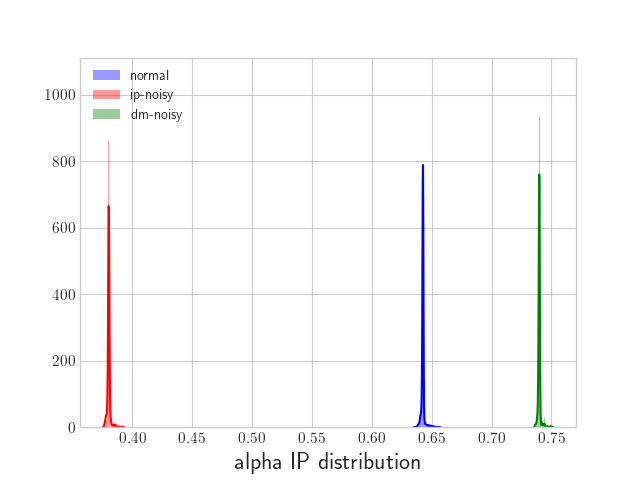
\includegraphics[width=\linewidth]{figures/alpha-distrib-low-cap}
\end{subfigure}%
\begin{subfigure}{.5\textwidth}
  \centering
  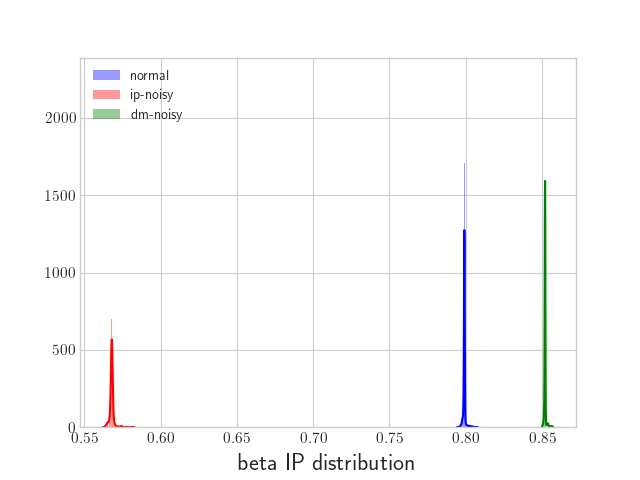
\includegraphics[width=\linewidth]{figures/beta-distrib-low-cap}
\end{subfigure}
\end{figure}


\subsection*{Robustness generalisation}
\begin{figure}[!h]
\centering
\begin{subfigure}{.5\textwidth}
  \centering
  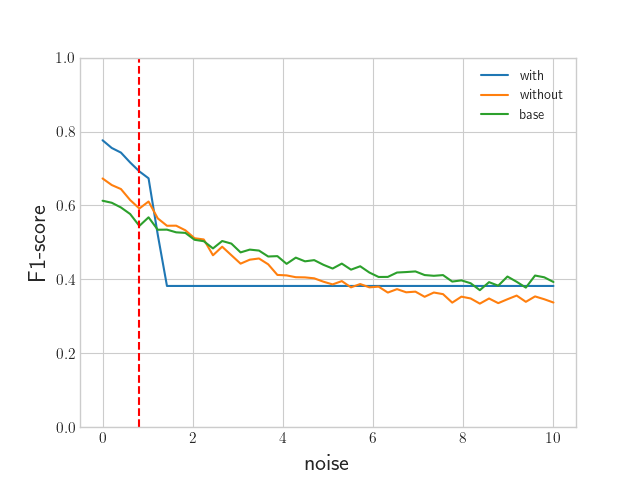
\includegraphics[width=\linewidth]{figures/noise-generalisation-bad-model-0}
\end{subfigure}%
\begin{subfigure}{.5\textwidth}
  \centering
  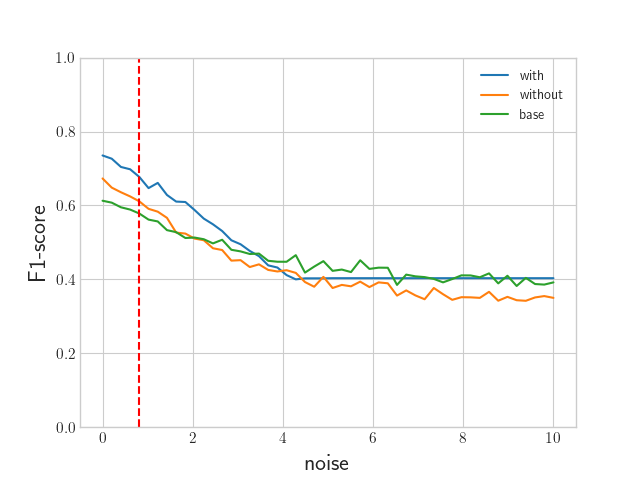
\includegraphics[width=\linewidth]{figures/noise-generalisation-good-model-6}
\end{subfigure}
\end{figure}

\subsection*{Yerkes-Dodson curve}
over-under arousal. do on larger range.
\begin{figure}[!ht]
\centering
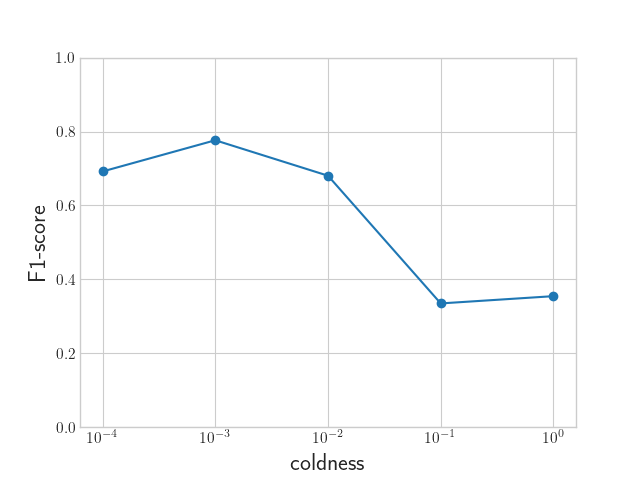
\includegraphics[scale=0.5]{figures/yerkes-dodson}
\end{figure}

\subsection*{Energy generalisation}
\begin{figure}[!ht]
\centering
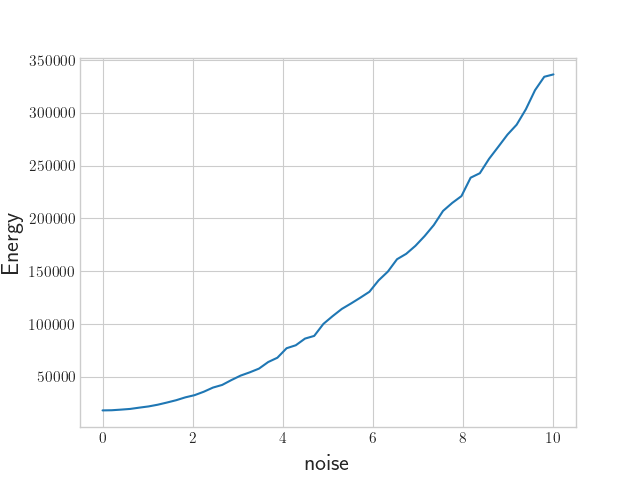
\includegraphics[scale=0.5]{figures/total-energy-model-1}
\end{figure}

